% LaTeX template for ENGR1000J-S2 Summer 2025 Final Project Report
\documentclass{engr1000j-s2}

% Main content
\begin{document}
  \thispagestyle{firstpage}
  
\includegraphics[height=0.75in]{figures/sjtubannerblue.png}
  \newline
  \newline
  \textbf{\Large ENGR1000J/VG100 Introduction to Engineering, Summer 2025}\\[0.5em]
  \textbf{{\Large \today}}

  \begin{center}
    \begin{minipage}{0.45\textwidth}
      
\includegraphics[height=0.8in]{figures/team logo.png}
    \end{minipage}\hfill
    \begin{minipage}{0.45\textwidth}
      \textbf{\Large Group 0: TC team}
    \end{minipage}\\[0.2em]
  \end{center}

  \noindent
  {\color{gray!30}\rule{\textwidth}{0.1pt}}

  {\Huge Project Title}

  \begin{center}
    
\includegraphics[height=3.5in]{figures/preface_picture.png}
  \end{center}

  \hspace{1em}

  % Team members
  { \Large \setlength{\parskip}{5pt} \setlength{\baselineskip}{0pt} Team Member${}^{1}$ (\begin{CJK}{UTF8}{gbsn}中文名\end{CJK}), \textit{\underline {email@address}}

  Zeyi Chen${}^{1}$ (\begin{CJK}{UTF8}{gbsn}陈泽奕\end{CJK}), $\textit{\underline{\href{mailto:marzich_44@sjtu.edu.cn}{marzich\_44@sjtu.edu.cn}} }$

  Xinchang Wang${}^{1}$ (\begin{CJK}{UTF8}{gbsn}王欣畅\end{CJK}), $\textit{\underline{\href{mailto:wang_xinchang@sjtu.edu.cn}{wang\_xinchang@sjtu.edu.cn}} }$

  Different Institute Member ${}^{2}$, \textit{\underline {email@address}}

  }

  \newpage
  \pagestyle{mystyle}
  % Abstract
  \section*{Abstract}
  \phantomsection
  \addcontentsline{toc}{section}{Abstract}
  This section includes information for those readers who will not read the entire
  document. Although this section appears first in the document, it is usually written
  last. It is one-paragraph long (not an introduction) and complete in itself (no
  reference numbers). It should indicate the general engineering background of your
  project and state the objectives. The design methodology, measurement techniques,
  observed facts, key understandings and conclusions must be stated in summary form.
  It should include a description of the project background, the project aim,
  the major tasks undertaken, the measurement techniques employed, key
  observations and physical understanding, conclusion and the significance of your
  findings. Word count is 200-400.

  \hspace{1em}

  % Acknowledgments
  \section*{Acknowledgments}
  \phantomsection
  \addcontentsline{toc}{section}{Acknowledgments}
  Thank all parties who assisted this project, such as TAs, instructors, companies,
  and teammates. Individuals other than the authors who contributed to the underlying research may be acknowledged in this section. The use of special facilities and other resources also may be acknowledged.

  % Table of Contents
  \newpage
  \tableofcontents
  \thispagestyle{mystyle}
  \newpage

  % Main sections
  \section{Introduction}
  This section gives the reader a flavor of the work or project presented: the
  context of the work, the objectives, scope. In another word, the problem, the need,
  and the solution. Normally it begins with more general background, then
  gradually narrows down to a particular problem. After clearly identify the problem,
  what is needed will be liberated followed by a solution (brief summary of what
  your prototype can offer). The main goal of this section is to establish the significance
  of your project--why is it needed. (page limit 2 pages)

  Background is where you set the context for your work. You need to place your work
  in a context beyond the immediate engineering application. Current societal
  topics are a good place to start: security, energy, sustainability,
  productivity, etc. Spend some time discussing the broader engineering issues, then
  gradually narrow the discussion down to the technical side of your project.
  Background can include reasonable technical discussions on some fundamental
  theories related to your project. Please avoid your own personal opinion and keep
  all the discussions objective.

  Proper citation is always required per academic ethic and HC. List and number all references at the end of the report. Corresponding bracketed numbers are used to cite references in the text \cite{vatistas1986reverse}, including citations that are an integral part of the sentence (e.g., ``It is shown in \cite{dornheim1996planetary} that\ldots '') or follow a mathematical expression: ``$A^{2} + B = C$ (Ref.~\cite{terster1997nasa}).'' For multiple citations, separate reference numbers with commas \cite{peyret2012computational,oates1997aerothermodynamics}, or use a dash to show a range \cite{volpe1994techniques,thompsonspacecraft,chi1993fluid,brandis2016nonequi}. Reference citations in the text should be in numerical order. 





  \hspace{1em}

  \textbf{Statements}
  \begin{itemize}
    \item Problem: clearly and concisely sums up what is the problem.\\

    \item Need/s: clearly and concisely sums up what is/are needed.\\

    \item Solution/s: clearly and concisely sums up the solution your project
      offers.
  \end{itemize}

  \hspace{1em}

  \section{Project Management}

  This section describes how your team managed this project. It should include a
  simple Gantt Chart, material budget, personnel information and contribution,
  and risk assessment. The tasks stated in the Gantt Chart correspond to the needs/solutions
  of this project.

  A Gantt chart provides concise but accurate information on the expected timetable
  for the project. The time for completion of each task should correspond
  exactly to the tasks previously described. Keep your Gantt Charts simple; as
  this graphic is intended for external audience, do not include too many tasks or
  descriptions of each task. An example is shown in Fig.~\ref{fig:gantt_chart}.

  Budget: State the proposed costs and budget of the project. Also include information
  on how you intend to manage the budget. One common way of showing the budget
  is according to the tasks as in Table \ref{tab:budget}.

  In building a set-up or prototype, material costs are typically accounted for in
  a bill of materials (BOM). This typically takes the form of the example shown
  below in Table \ref{tab:bill_of_materials}. State the costs of the project in an
  itemized form. Use a table, and make sure you list the total and any relevant sources
  for your purchases. If the purchasing link list is too long to fit in the main
  report body, you may include them as an appendix or a supplementary session.

  \begin{figure}[H]
    \centering
    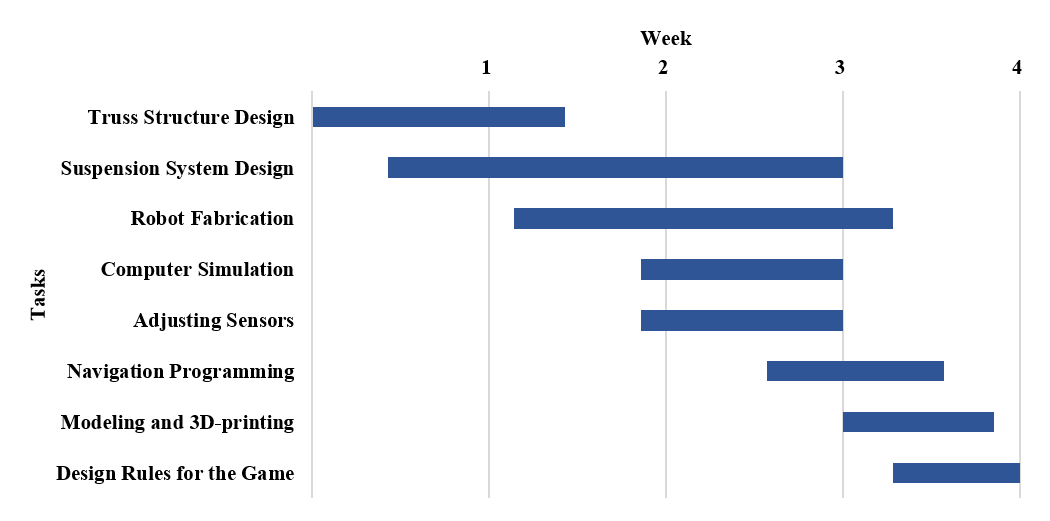
\includegraphics[width=0.8\textwidth]{figures/gantt_chart.png}
    \caption{\quad \textbf{Gantt chart for the project.}}
    \label{fig:gantt_chart}
  \end{figure}

  \begin{table}[H]
    \centering
    \caption{\quad \textbf{Project estimated budget}}
    \begin{tabular}{ p{0.15\textwidth} >{\centering\arraybackslash}p{0.45\textwidth}
    >{\centering\arraybackslash}p{0.3\textwidth} }
      \hline
      \hline
      Task       & Description of work                 & Anticipated costs, Yuan \\
      \midrule 1 & 3D-printing container               & 150.00                  \\
      2          & Construction of suspension system   & 100.00                  \\
      3          & Realisation of automatic navigation & 200.00                  \\
      4          & Construction of jogging system      & 200.00                  \\
      5          & Realisation of additional function  & 200.00                  \\
      6          & Tools                               & 150.00                  \\
      \hline
      \hline
                 & Total                               & 1000.00                 \\
    \end{tabular}
    \label{tab:budget}
  \end{table}

  Personnel: List the key personnel responsible for completion of the project, as
  well as other personnel involved in the project. Include brief summaries of
  their principal roles. These roles/contributions listed for each personnel shall
  be coherent with the tasks shown in Gantt Chart. The contributions of each
  team member are to be in agreement among the complete team, therefore, a
  signature is required from each member to endorse the content. (See Table
  \ref{tab:personnel} for an example.)

  

  \begin{table}[H]
    \centering
    \begin{threeparttable}
      \caption{\quad \textbf{Bill of materials}}
      \label{tab:bill_of_materials}
      \begin{tabular}{ p{0.10\textwidth} >{\centering\arraybackslash}p{0.30\textwidth}
      >{\centering\arraybackslash}p{0.15\textwidth} >{\centering\arraybackslash}p{0.15\textwidth}
      >{\centering\arraybackslash}p{0.15\textwidth} }
        \hline
        \hline
        Quantity   & Part Description & Purchased From\tnote{*} & Part Number & Price (Each in RMB) \\
        \midrule 8 & Wheel            & Vendor1                 & --          & 5.70                \\
        \dots      & \dots            & \dots                   & \dots       & \dots               \\
        \hline
        \hline
                   &                  &                         & Total =     & 1000.00
      \end{tabular}
      \begin{tablenotes}
        \item[*] The links are shown in the appendix.
      \end{tablenotes}
    \end{threeparttable}
  \end{table}

  \begin{table}[H]
    \centering
    \caption{\quad \textbf{Key personnel responsible for the project and their
    contributions}}
    \begin{tabular}{ p{0.25\textwidth} >{\centering\arraybackslash}p{0.40\textwidth}
    >{\centering\arraybackslash}p{0.25\textwidth} }
      \hline
      \hline
      Member             & Contributions                     & Signature                                            \\
      \midrule Ting Sun* & Specific contribution of Ting Sun & Sign here to acknowledge and agree with the content. \\
      Zeyi Chen          &                                   &                                                      \\
      Xinchang Wang      &                                   &                                                      \\
      \dots              & \dots                             & \dots                                                \\
      Member Name        &                                   &                                                      \\
      \hline
      \hline
    \end{tabular}
    \label{tab:personnel}
  \end{table}

  Risk Assessment: What needs to be in place for your project to succeed? What are
  the major sources of risk and how will you attempt to mitigate them? What is
  your fallback plan? What might be safety concerns?

  \section{System Design and Assembly}
  This section documents detailed design methodology and assembly procedure (concisely!)
  for your project. A schematic diagram of your overall system should be provided.
  The function and technical information about the key components should be
  explained in detail. You should present your step-by-step design procedure and
  the theory behind. Some photos, diagrams, and mathematical equations might be
  necessary. Readers should be able to re-create your system based on this section.
  You will be graded on the technical completeness of these descriptions.

  An example layout:

  \begin{itemize}
    \item Overall structure design (All components in your design including Fig.~\ref{fig:overall_design} and Fig.~\ref{fig:explosive_view})\\

    \item Key components and assembly (The part you want to explore in the discussion part)\\

    \item Electrical/circuit design (The workflow of your system including a block diagram. e.g. Fig. \ref{fig:block_diagram})
  \end{itemize}

  \begin{figure}[H]
    \centering
    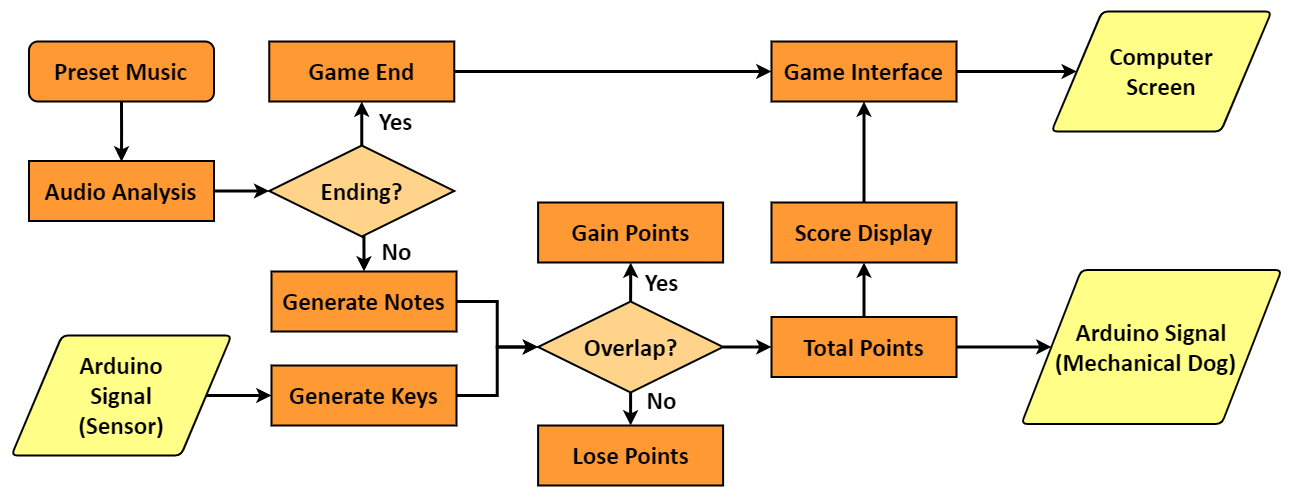
\includegraphics[width=\textwidth]{figures/block_diagram_sample.png}
    \caption{\quad \textbf{The workflow of the design.} (Generated by draw.io)}
    \label{fig:block_diagram}
  \end{figure}

  \begin{figure}[H]
    \centering
    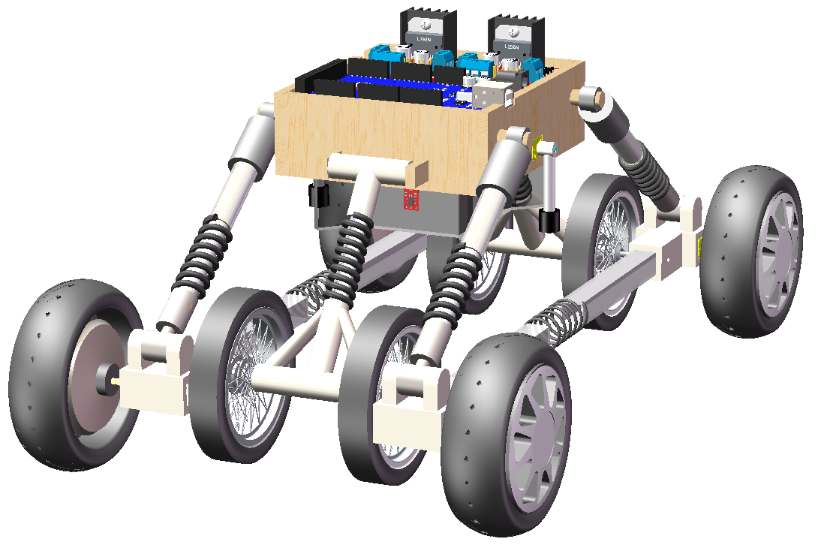
\includegraphics[width=0.8\textwidth]{figures/overall_design.png}
    \caption{\quad \textbf{The overall design of the explorer.} (Generated by
    SOLIDWORKS 2019)}
    \label{fig:overall_design}
  \end{figure}

  \begin{figure}[H]
    \centering
    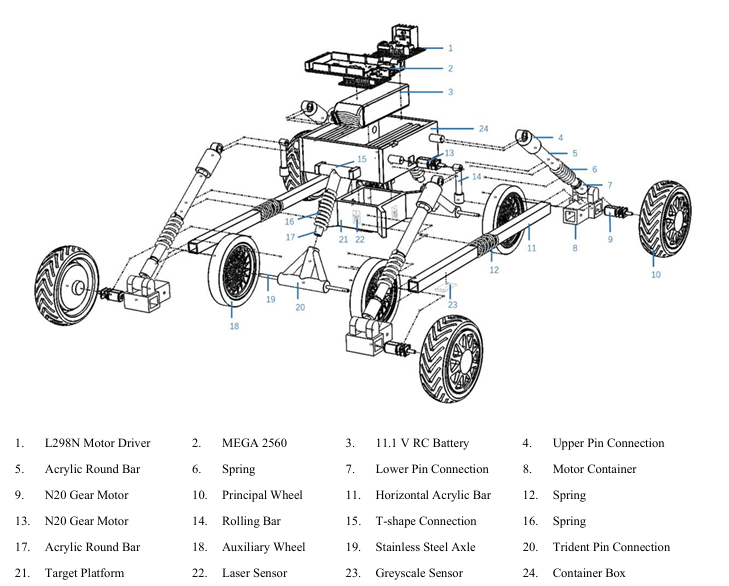
\includegraphics[width=\textwidth]{figures/explosive_view.png}
    \caption{\quad \textbf{Exploded view of the explorer.} (Generated by SOLIDWORKS
    2019)}
    \label{fig:explosive_view}
  \end{figure}

  

  \section{Measurement Results and Discussion}
  In this section you present your performance measurement results along with supporting
  text which ensures that the reader understands the data (description of post-processing
  or evaluation methods, analysis of uncertainties, exposition of tables/figures,
  correlations).

  Next is the most important part of the report – you are expected to assess
  critically what your results mean, what design implication they might have to the
  engineering community, and whether they make sense according to what you
  learned from the engineering lectures. Do not simply repeat in words what is obvious
  from your figures and tables (this is, sadly, a common mistake).

  

  Refer to a figure or a table by its number, not “figure below” or “table above.”
  When citing a figure in the text, use the abbreviation “Fig.” except at the beginning
  of a sentence. Do not abbreviate “Table”. Place a figure or a table close to (often
  immediately before or after) the “paragraph” of its first mention. By contrast,
  it is not necessary --- and so DO NOT place a figure or a table immediately after
  the “sentence” of the first mention; doing so inevitably breaks up a coherent
  paragraph (consisting of a topic sentence, several sentences of analysis and
  evidence, and a concluding remark) into several incoherent “paragraphs,” some
  made of a single sentence.

  Figures should have no background, borders, or outlines. Captions are bold with
  a single tab (no hyphen or other character) between the figure number and figure
  description. Keep the lettering size and style uniform both within each figure
  and throughout all of your illustrations. An example Figure is shown in Fig.
  \ref{fig:graph}.

  \begin{figure}[H]
    \centering
    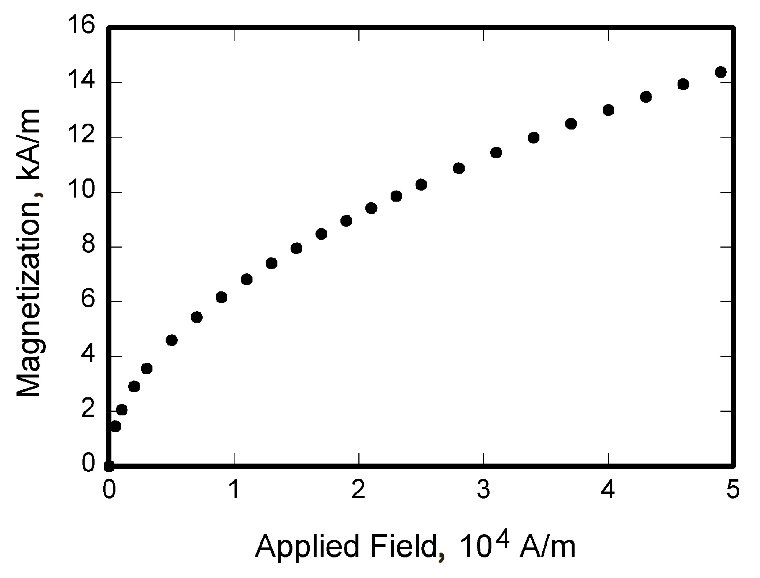
\includegraphics[width=.5\textwidth]{figures/graph.jpg}
    \caption{\quad \textbf{Magnetization as a function of applied fields.}}
    \label{fig:graph}
  \end{figure}

  Equations are numbered consecutively, with equation numbers in parentheses flush right, as in Eq.~\eqref{sample:equation}. Insert a blank line on either side of the equation. To insert an equation into the \LaTeX{} document, use the \verb|\begin{equation}...\end{equation}| command environment.

A sample equation is included here, formatted using the preceding instructions:

\begin{equation}
\label{sample:equation}
\int^{r_2}_0 F(r,\varphi){\rm d}r\,{\rm d}\varphi = [\sigma r_2/(2\mu_0)]\int^{\infty}_0\exp(-\lambda|z_j-z_i|)\lambda^{-1}J_1 (\lambda r_2)J_0 (\lambda r_i\,\lambda {\rm d}\lambda)
\end{equation}

Be sure that symbols in your equation are defined immediately following the equation. Also define abbreviations and acronyms the first time they are used in the main text.

  \section{Conclusions}
  Although a conclusion may review the main points of the report, do not
  replicate the abstract as the conclusion. Start with a concise summary of what
  you achieved in the project. You should cover the following points: What were the
  highlights of the project? How successfully did you meet your objectives? Where
  and why did you fail to meet objectives? How did your actual progress match
  your original plan? Was your estimating of time and resource accurate? With
  the benefit of hindsight, were there risks for which you failed to prepare adequately?
  Also discuss any problems which you encountered with e.g. equipment, shortage
  of resources (expertise/materials/etc.) or events/circumstances external to the
  project.

  Finally, explain how you achieved the learning outcomes for the project, listed
  in the module description. You may also offer a concise summary of further
  opportunities created by your work. Discuss any lessons to be learned for the benefit
  of future students.

  \hspace{1em}
  
  \bibliography{sample}

  In the reference list, give all authors' names; do not use ``et al.''. Papers that have not been published should be cited as ``unpublished''; papers that have been submitted or accepted for publication should be cited as ``submitted for publication.'' Private communications and personal website should appear as footnotes rather than in the reference list.

  References should be cited according to the standard publication reference style. Names and locations of publishers should be listed; month and year should be included for reports and papers. For papers published in translation journals, please give the English citation first, followed by the original foreign language citation.

  The examples below illustrate different reference types following the AIAA
  journal article traditions. All references should be in 9-point font, with
  reference numbers in brackets. \textbf{You are not required to indicate the type of reference;}
  different types are shown here for illustrative purposes only.

  The DOI (digital object identifier) should be incorporated in every reference
  for which it is available (see Ref.~\href{https://doi.org/10.1234/example.doi}{1}
  sample); for more information on DOIs, visit \href{https://www.doi.org}{www.doi.org}
  or \href{https://www.crossref.org}{www.crossref.org}.

  

  Note: The subtitles in this reference guide (e.g., "Periodicals," "Books," etc.)
  are for instructional purposes only. \textbf{They are NOT expected to show up in your
  final report.}

  \newpage
  %\appendix
  \section{Appendix}
  Additional materials and data.

  \newpage
  \section{Supplementary}
\end{document}